\documentclass[11pt]{article}
\usepackage[margin=1in]{geometry}
\usepackage[T1]{fontenc}
\usepackage{textcomp}
\usepackage{amsmath,amssymb,booktabs,graphicx,setspace,caption,threeparttable}
\usepackage[round,authoryear]{natbib}
\usepackage[hidelinks]{hyperref}
\captionsetup{font=small,labelfont=bf}
\onehalfspacing
\newcommand{\fignote}[1]{\par\vspace{2pt}{\footnotesize\emph{Notes:} #1\par}}

\title{\textbf{Operational Reliability of a Gas-Constrained Thermal Fleet:\\ Evidence from Five Years of Unit-Level Dispatch Reports in Bangladesh}}
\author{Tanvir Thamid\thanks{Independent researcher. E-mail: tanvirthamid@gmail.com. All data are public: the daily reports of the National Load Dispatch Centre published by the Bangladesh Power Development Board, NASA POWER weather data, BPDB annual reports and the WRI Global Power Plant Database. The code that collects, parses and analyses them is archived with the paper. \emph{Declaration of generative AI use:} a generative AI system (Claude, Anthropic) was used extensively in this work, to write and run the code for data collection, parsing and statistical analysis and to draft and edit the manuscript. The author directed the research, reviewed the analysis and the text, and takes full responsibility for the content of the paper.}}
\date{November 2026}

\begin{document}
\maketitle
\begin{abstract}
\noindent Reliability statistics for power plants in low- and middle-income countries are rarely published at the level of the generating unit. This paper builds a unit-day panel of Bangladesh's grid-connected fleet from 2,578 daily reports of the National Load Dispatch Centre (October 2019 -- November 2026): 409,000 unit-days for 225 units, each with capacity, evening-peak output, daily energy and the operator's stated reason for any shortfall, together with 1,618 generator trips described in the same reports. Parsed energy matches the reports' printed national totals on every checkable day, and inferred fuels match the official generation-by-fuel table within 2\%. The stated reasons behave as their meaning implies: capacity idled for gas shortage moves with daily gas supply ($r=-0.39$ within month) while capacity out for faults does not ($r=-0.02$). For October 2019 -- December 2024, within technology and calendar month, privately owned large thermal units spent 62 fewer days per 1,000 in forced outage (mean 117), tripped 7.3 fewer times per 1,000 unit-days (mean 11.9) and returned to service 36\% faster after an outage than state-owned units; the gap holds for trips recorded by the grid operator and for a measure that ignores the plants' own labels. Within units, heavy rain raised trips, almost entirely through electrical and grid causes, while daily maximum temperature had no detectable effect on trips, forced outages or engine faults. Associations with unit age are not robust to the uncertainty in commissioning dates.

\medskip
\noindent\textbf{Keywords:} power plant reliability; forced outage rate; generator trips; ownership; weather; Bangladesh.
\end{abstract}

\newpage
\section{Introduction}

How often generating units fail, and why, is the raw material of power-system reliability analysis \citep{billinton1996reliability}. In North America these statistics are collected under common definitions \citep{ieee762} and have been used to show that failures are correlated with temperature and system conditions, with consequences for reserve requirements \citep{murphy2018adequacy,murphy2019timedependent,murphy2020temperature}. For most grids in low- and middle-income countries no comparable unit-level record is published. Planners and researchers work with annual plant factors or national totals, which mix three different things: units that cannot run because something is broken, units that cannot run because there is no fuel or no money to buy it, and units that are not needed.

Bangladesh is a case where the distinction matters. Installed capacity grew to about 25 GW by 2023 \citep{bpdb2023annual}, yet supply has repeatedly fallen short of demand because gas and imported fuel ran out, and much of the fleet sits idle while capacity payments continue \citep{ieefa2024fixing}. Whether the problem is fuel, finance or the machines themselves is a question of engineering as much as policy.

This paper builds the missing record from a public source. Every day the National Load Dispatch Centre (NLDC) of the Power Grid Company of Bangladesh issues a report, published by the Bangladesh Power Development Board (BPDB). Its second page lists every grid-connected generating unit with its capacity, evening-peak output, energy for the day and a short remark such as ``Gas shortage'', ``Engine problem'', ``Under maintenance'' or ``Reserve''. Its first page narrates the day's events, including generator trips with clock times and, often, causes. I collected all 2,578 reports available from October 2019 to November 2026, parsed them into a panel of 409,000 unit-days for 225 units, classified the remarks and trip causes, linked units to commissioning dates and locations, and added daily weather.

The paper makes three contributions. The first is the dataset and its validation. Aggregate series from the same reports have been compiled for demand forecasting \citep{hossain2025dataset}; the unit-level table, the remarks and the trip narratives have not been used. Parsed unit energy sums to the printed national total on every one of 2,575 checkable days, and inferred unit fuels reproduce the official generation-by-fuel table within 2\%. Free-text remarks are only useful if they mean what they say, and I test this against independent series: capacity idled for gas shortage tracks daily gas supply, capacity out for faults does not, and units are almost never called ``reserve'' on days of heavy load shedding.

The second contribution is a comparison of state-owned and private units. Within the same technology and calendar month, private large thermal units spend about half as many days in forced outage, trip about 60\% less often and return to service about a third faster. Because private producers are paid for availability and might describe outages favourably, I show that the gap is the same for trips recorded by the grid operator and for zero-output days counted whatever the label. The comparison is descriptive: it cannot separate ownership from the vintage and design of the units each sector built, nor from priority in gas allocation. It adds operational evidence to a large literature on ownership and performance \citep{megginson2001state}.

The third contribution concerns weather. Within units, heavy rain raises the probability of a trip, and the increase is concentrated in electrical and grid-related causes rather than in turbines, boilers or fuel supply. Daily maximum temperature, by contrast, has no detectable effect on trips, forced-outage onsets or engine faults. This differs from the temperature dependence found for forced outages in the United States \citep{murphy2019timedependent}, although the estimates are not precise enough to rule out a sizeable effect on trips at the hottest temperatures.

\section{Data}

\subsection{The daily reports}
BPDB's archive (\url{https://misc.bpdb.gov.bd/daily-generation-archive}) lists dated entries back to 2007, but files exist only from October 2019; earlier entries point to a placeholder. For each of the 2,578 days from 19 October 2019 to 18 November 2026 I downloaded the system summary (page 1) and the unit table (page 2). The reports describe the operating day before the publication date. One day is missing because the wrong sheet was uploaded.

The unit table lists, for each unit or plant, its owner (BPDB, the state generation companies, joint ventures, independent and rental producers, imports), its configuration (for example ``1*217+118'' for a gas and a steam turbine), present capacity, output at the evening peak, energy for the day, and a remark. I extracted rows from the text layer by scanning for a configuration followed by three numbers, which handles both the 2019--2024 and the 2025--2026 layouts; rows whose energy figure wraps onto the next line are rejoined. The median day has 159 rows. On all 2,575 days with a printed national total, the parsed energy and capacity sum to that total within 0.5\%.

\subsection{Units, fuels and technology}
Plant names change spelling across days and were reformatted when the layout changed in December 2024. I link rows into 225 units by name similarity and configuration, map short-lived name variants to the unit with the same configuration on nearby days, and merge 16 renames by hand. Technology (combined cycle, gas turbine, steam, reciprocating engine, solar, hydro, wind, import, nuclear) comes from names and configurations; fuel from names, a list of coal plants and the history of fuel-related remarks. For 650 days in 2025--26 the reports also give generation by fuel. Summing parsed unit energy by inferred fuel reproduces these totals within 2\% for every fuel (gas 0.994, coal 1.003, oil 0.982; hydro, solar, wind, imports and nuclear 1.000); 0.3\% of energy is not assigned a fuel.

Commissioning years for 107 thermal units come from the list of projects commissioned between 2010 and June 2023 in BPDB's annual report \citep{bpdb2023annual}, matched by hand because the report uses different names and per-unit capacities. Older units were dated from the Global Power Plant Database \citep{wri2021gppd} and from published sources checked individually (17 units); three remain uncertain and 30, mostly small engine plants, are undated. Units that first appear after November 2019 are dated by first appearance. Units are located at town level and assigned daily maximum temperature, relative humidity and precipitation from NASA POWER \citep{nasapower}. Against the maximum temperature printed in the 2025--26 reports for Dhaka, the NASA POWER series correlates at 0.82 and runs 1.4\,\textdegree C cooler, as expected for a grid-cell average.

\subsection{Outage causes}
The 1,055 distinct remarks were coded by keyword rules into gas shortage, other fuel shortage, payment or finance, fault (``engine problem'', ``machine problem'', trips, leaks), maintenance, reserve or low demand, grid constraint, contract expiry, test, water level, and running modes (frequency control) that carry no cause. Only 0.2\% of offline capacity-days remain unclassified. Consecutive days offline form an outage spell. Spells whose remarks only say ``under maintenance'' are classed as planned if a remark mentions an overhaul, inspection or scheduled work, as forced if a remark names a fault or a trip for that unit is recorded on the first day or the day before, and as unspecified otherwise. Forced spells last a median of 2 days and follow a day of running in 98\% of cases; planned spells last a median of 12 days.

Three checks support the coding. Daily capacity idled for gas shortage correlates with the reported gas supplied to power stations at $-0.39$ within calendar months (and $-0.64$ in levels), whereas capacity out for faults ($-0.02$), other fuels ($-0.01$) and maintenance ($-0.06$) does not move with gas. Capacity labelled reserve averages 2,080 MW on days without load shedding, 198 MW on days with up to 500 MW shed and 40 MW on days with more: units are not called spare while customers are being cut off.

A change in reporting in January 2025 left 33--41\% of idle capacity without a remark, against 4--13\% in 2024. The analysis therefore uses October 2019 -- December 2024.

\subsection{Generator trips}
The first page of each report narrates events of the previous day. I join continuation lines, keep items that report a trip of a generating unit (rather than of a line, transformer or bus), and extract the trip time, the resynchronisation time if given and the stated cause. This yields 1,618 generator trips, 1,543 of them linked to a unit. Causes are stated for 784 and coded as fuel supply (203), electrical (133), turbine (77), boiler or heat-recovery steam generator (67), grid (67), control and instrumentation (54), cooling water (27) and other (156). Because the narratives are written by the grid operator, trips are the measure least exposed to plants' own reporting.

\subsection{The fleet, 2019--2024}
Figure~\ref{fig:lost} shows the capacity not generating at the evening peak by stated cause. In 2019--2020 most idle capacity was reserve. From 2022 it was mostly fuel: gas shortage, and from 2023 shortages of oil and coal as foreign exchange ran short. Faults and maintenance account for a steady 1--3 GW. Table~\ref{tab:fleet} summarises the four thermal technologies. Combined-cycle units ran on 72\% of days and had a daily forced-outage rate of 0.07; single-cycle gas turbines ran on 45\% of days, were idle for fuel or as reserve on 31\%, and had a forced-outage rate of 0.24. Reciprocating engine plants appear as single rows of 10--30 engines, so a failed engine shows up as reduced output rather than as an outage; they are analysed through the share of capacity lost while running with a fault remark.

\begin{figure}[t]
\centering
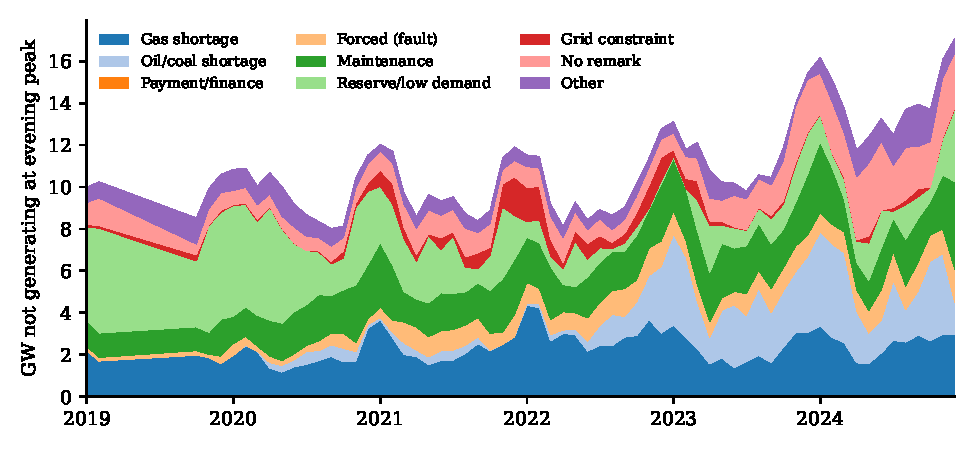
\includegraphics[width=\textwidth]{fig/fig1_lost_capacity.pdf}
\caption{Capacity not generating at the evening peak, by stated cause}\label{fig:lost}
\fignote{Monthly means of daily totals. For units that are off, their capacity; for units that are running, capacity minus evening-peak output, attributed to the unit's remark. All grid-connected units, October 2019 -- December 2024.}
\end{figure}

\begin{table}[t]
\centering\small
\caption{Thermal units by technology, October 2019 -- December 2024}\label{tab:fleet}
\begin{threeparttable}
\setlength{\tabcolsep}{4pt}\begin{tabular}{lrrrrrrrr}
\toprule
 & Units & Unit-years & Running & Fuel or & Forced & Maint. & Reserve & Daily \\
 & & & (\%) & finance (\%) & (\%) & unspec.\ (\%) & (\%) & FOR \\
\midrule
Combined cycle & 40 & 158 & 72.4 & 8.5 & 5.3 & 9.2 & 1.4 & 0.069 \\
Gas turbine & 24 & 112 & 44.6 & 15.3 & 14.0 & 5.3 & 15.3 & 0.239 \\
Steam & 19 & 60 & 45.5 & 26.0 & 2.1 & 22.8 & 0.9 & 0.044 \\
Reciprocating engine & 96 & 379 & 83.4 & 4.6 & 0.9 & 0.2 & 8.5 & 0.010 \\
\bottomrule
\end{tabular}
\begin{tablenotes}\footnotesize
\item Shares of unit-days by state. Daily FOR = forced days / (forced + running days). Remaining shares are planned maintenance, tests, grid constraints, contract expiry and days without a remark. For engine plants an outage of one engine does not appear as a unit outage.
\end{tablenotes}
\end{threeparttable}
\end{table}

\section{Methods}

Outcomes are measured per unit-day and expressed per 1,000 unit-days. For the effect of weather and system conditions I estimate, for the large thermal units (combined cycle, gas turbine, steam),
\begin{equation}
y_{it} = \sum_{k} \beta_k \, \mathbf{1}[T^{\max}_{it} \in k] + \gamma' X_{it} + \alpha_i + \delta_{m(t)} + \varepsilon_{it},
\end{equation}
where $y_{it}$ is a trip or the start of a forced outage, the sample is restricted to units that ran the day before, $k$ indexes bins of daily maximum temperature (reference 30--33\,\textdegree C), $X_{it}$ contains relative humidity, precipitation, system evening-peak demand relative to its monthly mean (GW) and an indicator for load shedding, $\alpha_i$ are unit fixed effects and $\delta_{m(t)}$ year-month fixed effects. The comparison is therefore within a unit and within a month, so that seasonal maintenance, fuel-supply regimes and the composition of the fleet are held fixed. For engine plants the outcome is the percentage of capacity lost while running with a fault remark.

For differences between units I replace unit fixed effects with technology-by-year-month fixed effects and include ownership (private versus state or joint venture), age bins and log capacity. Outcomes are the forced state (among days running or in forced outage), trips (among units that ran the day before) and non-fuel unavailability (off for a reason other than fuel, finance, reserve or contract expiry). Standard errors are clustered by unit throughout; alternatives are reported. Repair times are analysed with a Cox model of the hazard of returning to service for forced and unspecified-maintenance spells, with right-censored spells retained.

\section{Results}

\subsection{Ownership}
Table~\ref{tab:own} reports the comparison of private and state-owned units. Within technology and month, and holding age and size fixed, private units spent 62 fewer days per 1,000 in forced outage, against a mean of 117, were unavailable for non-fuel reasons 11.7 percentage points less often (mean 21.7) and tripped 7.3 fewer times per 1,000 unit-days (mean 11.9). Among combined-cycle units alone the forced-state gap is $-58.5$ (s.e.\ 23.8) on a mean of 69. After an outage, private units returned to service faster: the hazard ratio is 1.36 ($p=0.01$), controlling for technology, outage class, year, age and size.

\begin{table}[t]
\centering\small
\caption{Private versus state-owned large thermal units}\label{tab:own}
\begin{threeparttable}
\begin{tabular}{lccc}
\toprule
 & Forced state & Non-fuel unavailable & Trips \\
 & (per 1,000 days) & (\% of days) & (per 1,000 days) \\
\midrule
Private & $-61.8$ (27.8) & $-11.7$ (4.5) & $-7.3$ (3.4) \\
Age 0--4 years & $34.5$ (38.5) & $13.4$ (6.8) & $-2.9$ (3.9) \\
Age 10--19 years & $77.0$ (89.7) & $11.4$ (8.0) & $0.7$ (3.2) \\
Age 20+ years & $92.2$ (42.8) & $-8.0$ (5.8) & $-5.6$ (4.8) \\
Log capacity & $45.8$ (38.7) & $-3.2$ (5.0) & $3.1$ (2.1) \\
\midrule
Mean of outcome & 116.8 & 21.7 & 11.9 \\
Unit-days & 70,198 & 105,390 & 63,044 \\
Units & 79 & 81 & 76 \\
\bottomrule
\end{tabular}
\begin{tablenotes}\footnotesize
\item Linear probability models with technology $\times$ year-month fixed effects; reference age 5--9 years; standard errors clustered by unit in parentheses. Forced state: among days running or in forced outage. Trips: among units that ran the day before. Combined cycle, gas turbine and steam units with known commissioning year, October 2019 -- December 2024.
\end{tablenotes}
\end{threeparttable}
\end{table}

Private producers are paid capacity charges that depend on declared availability, so they may label outages differently. Two measures are not exposed to this. Trips are written down by the grid operator, and the trip gap is the same with standard errors clustered by plant site ($p=0.03$). A count of days with zero output for any reason other than fuel, finance, reserve or contract expiry, whatever the remark, gives a private gap of 15.3 percentage points (s.e.\ 4.8). Without the age control, so that undated units are included, the forced-state gap is $-84$ (31).

The comparison does not identify an effect of ownership. Within each technology, private and public units differ in vintage, manufacturer and design, and private gas plants may have received gas first. The estimates show that, in this fleet, private units were more available and more reliable in operation, by margins that survive the obvious reporting objection.

\subsection{Weather and system conditions}

\begin{figure}[t]
\centering
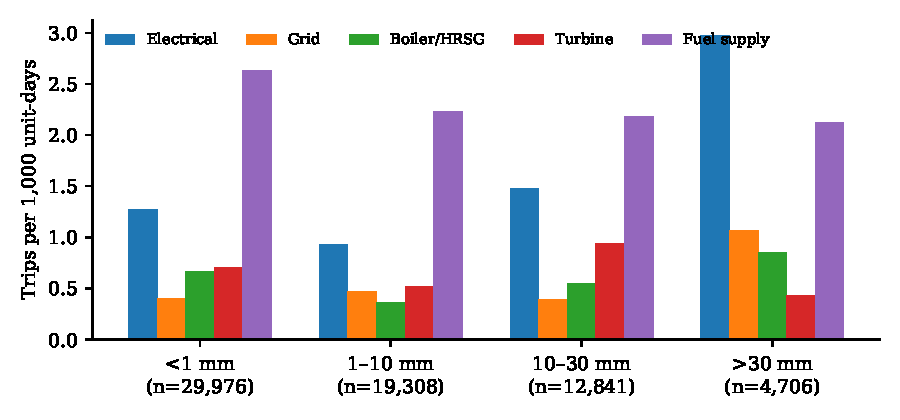
\includegraphics[width=0.92\textwidth]{fig/fig2_rain_causes.pdf}
\caption{Generator trips by stated cause and daily precipitation}\label{fig:rain}
\fignote{Large thermal units that ran the day before, October 2019 -- December 2024. Trips with unstated or other causes are not shown. Precipitation from NASA POWER at the unit's location.}
\end{figure}

Within units, precipitation raises the probability of a trip by 0.09 per 1,000 unit-days per millimetre (s.e.\ 0.03), against a mean of 11.9. The estimate is the same with lagged temperature, with unit-by-calendar-month fixed effects, without load-shedding days and with standard errors clustered by unit and date ($p$ between 0.004 and 0.02). On days with more than 30 mm, electrical trips occur 3.1 times per 1,000 unit-days against 1.2 on dry days, and grid-related trips 1.0 against 0.4, while turbine and fuel-supply trips do not change (Figure~\ref{fig:rain}). The pattern points to lightning, moisture in electrical equipment and faults on the transmission network rather than to the prime movers.

Temperature has no detectable effect (Figure~\ref{fig:heat}). Relative to days of 30--33\,\textdegree C, trips of large thermal units are 4.6 per 1,000 higher above 36\,\textdegree C (s.e.\ 3.2) and forced-outage onsets 3.0 lower (1.6). Per degree, trips rise by 0.44 per 1,000 (0.33) for all large thermal units and 0.80 (0.50) for combined-cycle units; for forced onsets and trips combined the coefficient is $-0.32$ (0.46). These estimates are stable across the specifications above. For engine plants, the share of capacity lost to engine faults does not vary with temperature ($-0.04$ percentage points per degree, s.e.\ 0.05). The data rule out large effects on forced-outage onsets but not on trips: for combined-cycle units above 36\,\textdegree C the 95\% interval for trips runs from $-2.7$ to $+16.4$ per 1,000, on a mean of 16.4.

System demand above its monthly mean is associated with fewer events: $-0.6$ to $-0.9$ per 1,000 per GW ($p<0.05$). This is more plausibly operational, with maintenance deferred and units held steady on days of high demand, than a physical effect, and I do not interpret it further.

\begin{figure}[t]
\centering
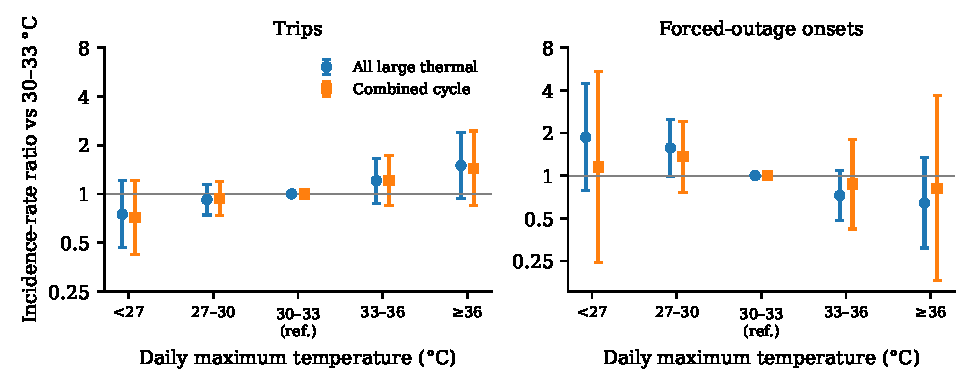
\includegraphics[width=\textwidth]{fig/fig3_heat.pdf}
\caption{Trips and forced-outage onsets by daily maximum temperature}\label{fig:heat}
\fignote{Coefficients on temperature bins from equation (1), with 95\% confidence intervals; reference 30--33\,\textdegree C. Unit and year-month fixed effects; controls for humidity, precipitation, demand deviation and load shedding; standard errors clustered by unit.}
\end{figure}

\subsection{Age and repair times}
In Table~\ref{tab:own}, units aged 20 years or more spend 92 more days per 1,000 in forced outage than units aged 5--9, and new units (under 5 years) are unavailable for non-fuel reasons 13 points more often, a pattern consistent with early-life failures. Neither result is robust. Restricted to units whose commissioning year is documented in the annual report or in checked sources, no age coefficient is significant, and correcting two commissioning dates during the work changed the raw forced-outage rate of the oldest units from 25\% to 8\%. Repair is slower for old units (hazard ratio 0.74, $p=0.05$), steam units (0.65, $p=0.03$) and larger units (0.76 per log MW). Where both times are reported, combined-cycle units resynchronised a median of 2.8 hours after a trip and steam units 3.5 hours.

\section{Discussion}

The daily dispatch reports of a national grid operator turn out to support reliability statistics at the level of the unit. Because the parsed figures reproduce the printed totals and the official fuel mix, and the stated causes co-move with independent series as their meaning implies, the remarks can be used to separate units that are broken from units that lack fuel. In Bangladesh between 2019 and 2024 the second dominated: from 2022 most idle thermal capacity at the evening peak was idle for gas, oil or coal.

The ownership gap is large and survives the most obvious objection, but it is a comparison of two fleets, not an experiment. A natural next step is to compare units of the same model and vintage across owners, which would require manufacturer data the reports do not contain. The rain result has a clear mechanism and is directly relevant to protection and lightning design at plants and substations; a lightning-flash dataset would allow a sharper test. The absence of a measurable heat effect contrasts with evidence from the United States \citep{murphy2019timedependent}; it may reflect the narrow range of temperatures in a humid tropical climate, the coarse temperature measure, or the dominance of fuel constraints, under which units that would be derated by heat are often not running.

Several limitations apply. The reports are snapshots at the evening peak with daily energy, so outages shorter than a day appear only as trips. Remarks are written by plants and by dispatchers and are not audited. ``Under maintenance'' cannot always be classified as planned or forced. Commissioning years are uncertain for the oldest units. And the reporting change of January 2025 limits the main sample to five years and three months.

\section{Conclusion}

Public daily reports from Bangladesh's grid operator yield a validated unit-level record of availability, outage causes and generator trips for a whole national fleet. Over 2019--2024, fuel rather than equipment was the main reason thermal capacity stood idle; private units were markedly more available and quicker to recover than state-owned units of the same technology; heavy rain raised electrical and grid-related trips; and no effect of daily heat on outages could be detected. The same approach could be applied wherever dispatch reports are published.

\bibliographystyle{plainnat}
\bibliography{refs}

\end{document}
